\section{Альтернативные решения}

\subsection{Инструменты}

\subsubsection{DeepFaceLab}

Одно из самых популярных решений в области замены лица - DeepFaceLab\cite{deepfacelab}. Оно существует с 2018 года и до сих пор остается передовой и активно развивающейся технологией.

Плюсами являются очень высокое качество наложения и хорошее сохранение похожести лица, большое количество возможностей для подстройки для конкретной пары лиц и видео, высокое разрешение лица.

Несмотря на преимущества, у DFL есть несколько серьезных недостатков, значительно усложняющих его использование. Для работы DFL требует дообучения модели для конкретной пары лиц на достаточно большом наборе данных, включающем изображения со всех ракурсов как для человека на видео, так и для накладываемого персонажа.
Так же дообучение занимает значительное время и требует больших мощностей.
DFL работает по принципу маски, накладывая одно лицо на другое, что делает его очень чувствительным к качеству датасетов. Так же это создает проблему разницы в освещении и цвете между видео и датасетом маски.

Упомянутые выше недостатки проявляются для потенциального пользователя в следующих минусах:

\begin{itemize}
    \item Необходимость в сборе большого (несколько десятков или более изображений) датасета для актера и накладываемого персонажа
    \item После сбора датасета необходимо дообучать модель в течение нескольких недель
    \item Датасет должен быть очень качественным, т.е. иметь изображения с разнообразных углов и с разным освещением
\end{itemize}

\subsubsection{FSGAN}

FSGAN\cite{nirkin2019fsgan}\cite{nirkin2022fsganv2} - более современная технология, появившаяся в 2019 году.

Face reenactment (перенос мимики, puppeteering) - использование движений и мимики лица в ведущем видео для управления мимикой и движением лица, представленном на другом видео или изображении.

Алгоритм работы FSGAN состоит из следующих шагов:

\begin{itemize}
    \item Сегментация - выделение лица на исходном и целевом изображении
    \item Face reenactment - воссоздание мимики и положения лица на целевом видео с исходным лицом
    \item Смешивание лиц (face blending) - наложение получившегося лица на целевое изображение с сохранением цвета кожи и освещения
\end{itemize}

Решение, предлагаемое FSGAN не требует дообучения для конкретных пар лиц и предлагает замену лица на основе лишь одного изображения исходного лица, против большого датасета для DeepFaceLab.

Тем не менее, FSGAN имеет довольно низкое качество наложения, так выглядит пример его работы:

\begin{figure}[H]
    \centering
    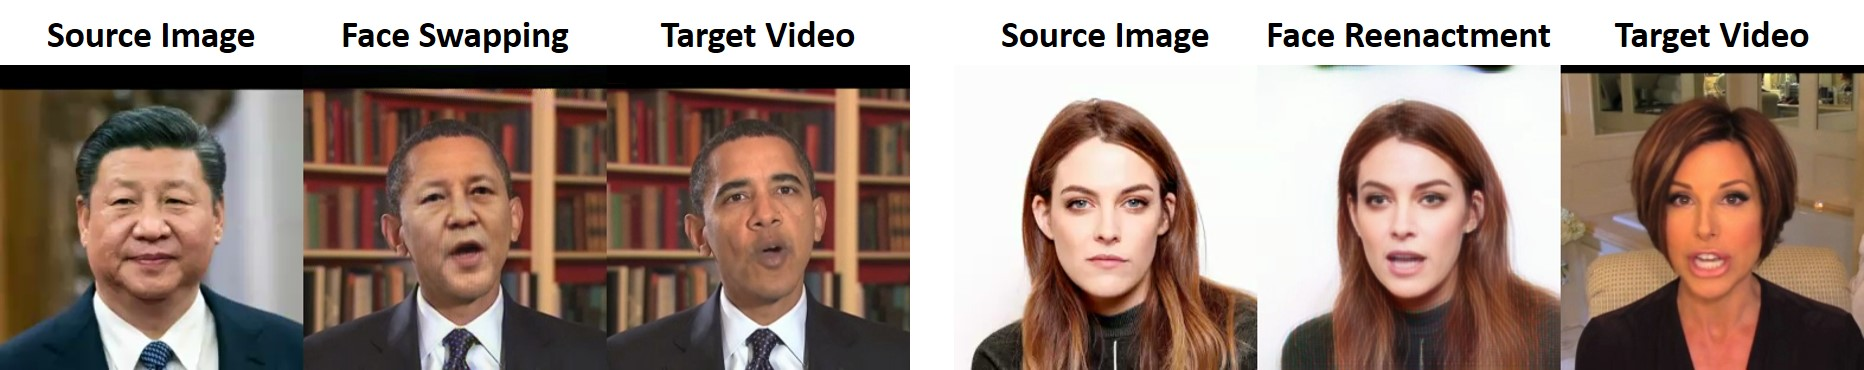
\includegraphics[width=0.8\linewidth]{fsgan_teaser.jpg}
    \caption{Примеры работы замены лица и переноса мимика в FSGAN} \label{fsgan_results}
\end{figure}

\subsection{Готовые сервисы}

\subsubsection{Reface}

Популярным сервисом для замены лица является Reface. Это приложение для смартфонов, позволяющее наложить свою фотографию на один из видеороликов, предоставленых Reface.
Приложение ориентировано на сегмент b2c, т.е. массового пользователя. Reface по очевидным причинам не подходит для создания видеоконтента для бизнеса.
Во-первых, лица можно накладывать только на ролики из существующего набора, который содержит отрывки из популярных фильмов и сериалов.
Во-вторых, выходное качество видео очень низкое - это касается как качества наложения, так и выходного разрешения, частоты кадров и других параметров видео.
Сервис ориентирован на то, что роликами просто будут делиться в соцсетях и мессенджерах, а не на серьезный видеопродакшн.

Минусы Reface исходят из его позиционирования на другой сегмент, и таким образом он не является хорошей альтернативой в сегменте b2b.

\subsubsection{Другие мобильные приложения}

Помимо Reface похожие функции появляются во многих других мобильных приложениях. Все они ориентированы на сегмент b2c, имеют низкое качество выходного видео и множество ограничений.
Большая часть таких приложений накладывает лица только на фотографии, но не видео.